\documentclass{article}

\usepackage[utf8]{inputenc}
\usepackage{geometry}
\usepackage{listings}
\usepackage{graphicx}
\usepackage{geometry}
\usepackage{courier}

\graphicspath{{../images/}}

\title{HW 5 \\ Serial Mandelbrot}
\author{Philip Nelson}
\date{2018 October 1}

\lstset{basicstyle=\footnotesize\ttfamily\normalsize,
        breaklines=true,
        stepnumber=1,
       }

\begin{document}

\maketitle

\section*{Introduction}

The purpose of this assignment is to write an MPI program that generates an image of the mandelbrot set as described by the set of complex numbers $c$ for which the function ${f_{c}(z)=z^{2}+c}$ does not diverge when iterated from $z=0$. My program takes as input the image height, image width, maximum number of iterations, minimum x/real value, maximum x/real value, and minimum y/imaginary value. It then calculates the number if iterations every pixel in the image takes to diverge and stores those values in an array. When every pixel has been calculated, the array is converted to a bitmap image based on a color scheme. Functionality to output to a ppm file is included.

\section*{Code}
The code is broken up into four main files, main.cpp, calculator.cpp, color.cpp, and ppmToBmp.hpp. The files are included below.

\bigskip

\subsection{main.cpp}
\lstinputlisting[showstringspaces=false, language=c++, numbers=left]{../main.cpp}

\subsection{calculator.cpp}
\lstinputlisting[showstringspaces=false, language=c++, numbers=left]{../calculator.cpp}

\subsection{color.cpp}
\lstinputlisting[showstringspaces=false, language=c++, numbers=left]{../color.cpp}

\subsection{ppmToBmp.hpp}
\lstinputlisting[showstringspaces=false, language=c++, numbers=left]{../ppmToBmp.hpp}
\newpage
\section*{Output}

\begin{lstlisting}[showstringspaces=false]

# mpic++ -std=c++17 -g0 -O3 -Wall -Wextra -Werror main.cpp calculator.cpp color.cpp -o mandelbrot.out

# mpiexec -n 4 ./mandelbrot.out 2048 2048 1000 -.760574 -.762574 -.0837596

Writing brot.bmp...
Success!
2048 x 2048
Time to compute: 4.26297
Time to write image: 0.244798
Total time: 4.50777

\end{lstlisting}

\section*{Findings}

I generated the image below, Figure \ref{fig:image}, as a 256x256, 512x512, 1024x2014, 2048x2048, 4096x4096, and 8192x8192 pixel image. I ran each size 10 times and took the average time to calculate the number of iterations for each pixel and the time to write the file to the disk. The results are detailed in Figure \ref{fig:graph}. The graph shows that the time to generate an image increases with the square of the number of pixels. The same is true for the writing of the file to the disk. Another interesting metric can be seen in Figure: \ref{fig:graph2} which shows how the pixels per second calculated was not largely affected by the image size. You can however see that it slowly increases with larger images. I believe this is due to caching.

\begin{figure}[!htbp]
    \centering
    \fbox{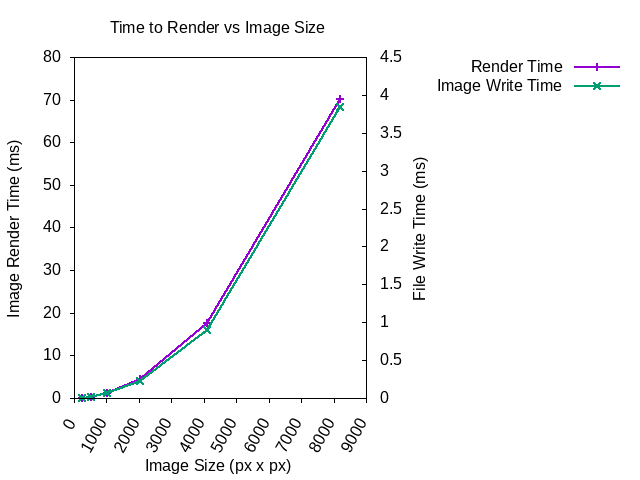
\includegraphics[width=150mm]{benchmark.png}}%tabe size
    \caption{}
    \label{fig:graph}
\end{figure}

\begin{figure}[!htbp]
    \centering
    \fbox{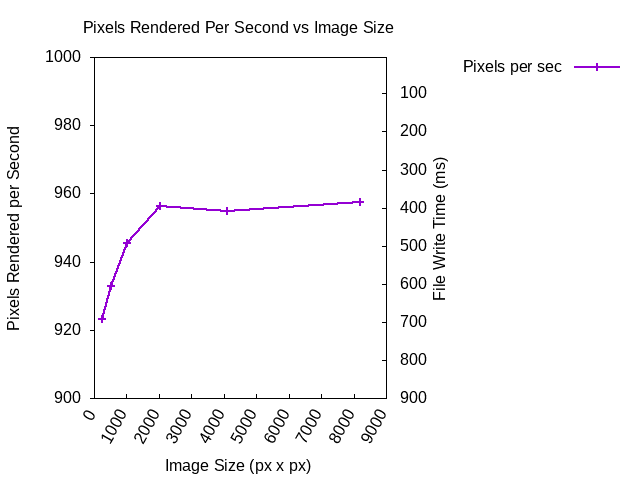
\includegraphics[width=150mm]{pixelsPerSec.png}}%tabe size
    \caption{}
    \label{fig:graph2}
\end{figure}

\begin{figure}[!htbp]
    \centering
    \fbox{
\includegraphics[width=150mm]{spiral.png}}%tabe size
    \caption{}
    \label{fig:image}
\end{figure}

\end{document}
